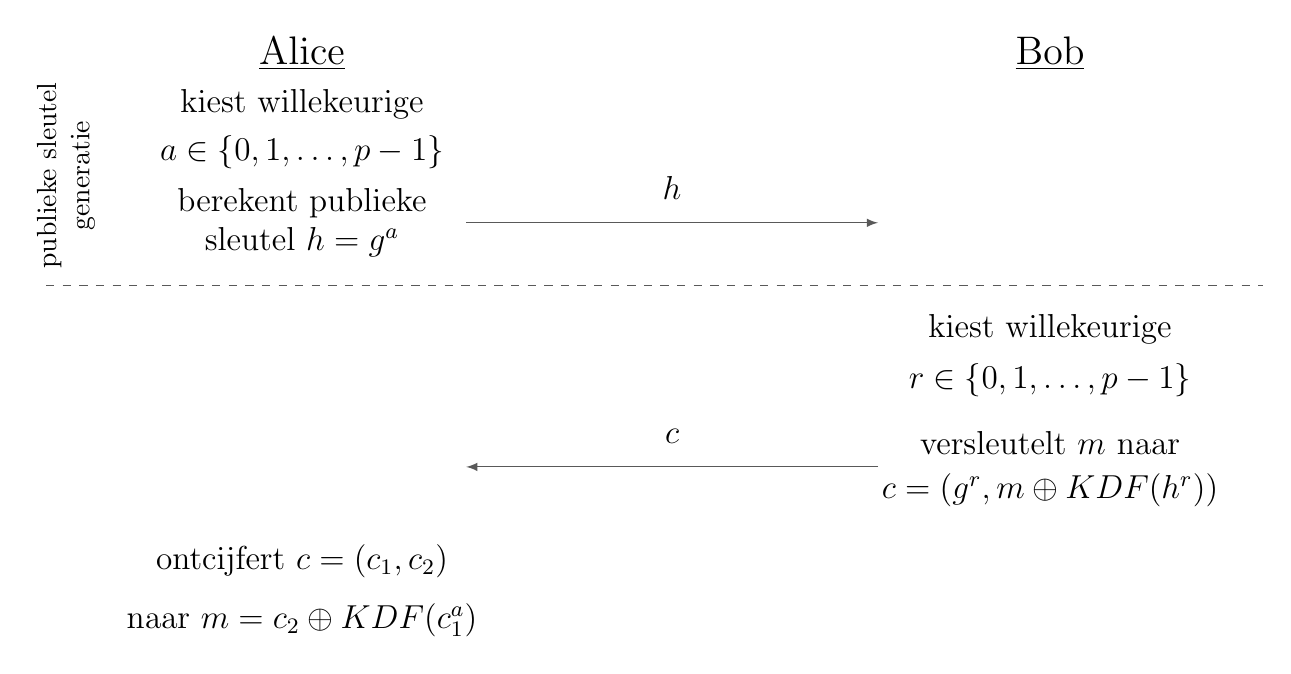
\begin{tikzpicture}[
    >=latex,
    textline/.style={
        font=\large,
        align=center
    },
    person/.style={
        font=\Large
    },
    formula/.style={
        font=\large
    },
    message/.style={
        ->,
        draw=black!65,
        thin,
        shorten >=1pt,
        shorten <=1pt
    },
    separator/.style={
        draw=black!65,
        thin,
        dashed
    }
]

% Horizontal positions
\def\AliceX{0}
\def\BobX{9.5}

% ==================================================
% Participants
% ==================================================

\node[person] at (\AliceX,5.2)
    {\underline{Alice}};

\node[person] at (\BobX,5.2)
    {\underline{Bob}};

% ==================================================
% Public-key generation
% ==================================================

\node[
    rotate=90,
    textline,
    font=\normalsize,
    align=center
] at (-3.0,3.65)
    {publieke sleutel\\generatie};

\node[textline] at (\AliceX,4.55)
    {kiest willekeurige};

\node[formula] at (\AliceX,3.95)
    {$a\in\{0,1,\ldots,p-1\}$};

\node[textline] at (\AliceX,3.05)
    {berekent publieke\\sleutel $h=g^a$};

% Alice sends the public key h to Bob
\draw[message]
    (2.05,3.05)
    --
    node[above=5pt, font=\large] {$h$}
    (7.35,3.05);

% ==================================================
% Separator
% ==================================================

\draw[separator]
    (-3.25,2.25) -- (12.2,2.25);

% ==================================================
% Encryption by Bob
% ==================================================

\node[textline] at (\BobX,1.70)
    {kiest willekeurige};

\node[formula] at (\BobX,1.05)
    {$r\in\{0,1,\ldots,p-1\}$};

\node[textline] at (\BobX,0.25)
    {versleutelt $m$ naar};

\node[formula] at (\BobX,-0.35)
    {$c=\bigl(g^r,m\oplus KDF(h^r)\bigr)$};

% Bob sends ciphertext c to Alice
\draw[message]
    (7.35,-0.05)
    --
    node[above=5pt, font=\large] {$c$}
    (2.05,-0.05);

% ==================================================
% Decryption by Alice
% ==================================================

\node[textline] at (\AliceX,-1.25)
    {ontcijfert $c=(c_1,c_2)$};

\node[textline] at (\AliceX,-2.00)
    {naar $m=c_2\oplus KDF(c_1^a)$};

\end{tikzpicture}